\documentclass[12pt, letterpaper, oneside]{book}
\usepackage{pseudocode}
\usepackage{amsfonts}
\usepackage{amsmath}
\usepackage{amssymb}
\usepackage{csquotes}
\usepackage{float}
\usepackage{hyperref}
\usepackage[letterpaper, textwidth=7.5in, textheight=8in]{geometry}
\hypersetup{
  colorlinks=true,
  linkcolor=blue,
  filecolor=magenta,
  urlcolor=blue,
}
\usepackage{tikz}
\usetikzlibrary{arrows, automata, positioning, shapes.geometric}
\usepackage{titlesec}
\usepackage{parskip}
\usepackage{xcolor}

\setcounter{secnumdepth}{4}

\title{
  Notes on \textit{Introduction to Lattices and Order (2nd edition)}
}
\author{Yaobin Wen}
\date{Jan 2024}

\begin{document}

\maketitle
\tableofcontents

\chapter*{Overview}
\addcontentsline{toc}{chapter}{Overview}

This document contains my study notes of the textbook \textit{Introduction to Lattices and Order (Second edition)} by
B.A.Davey and H.A. Priestley. I use it for a few purposes:

\begin{enumerate}
  \item As a reference to quickly refresh my memory on the subjects.
  \item Keep the notes to help me understand the text that is not obvious for
        me to comprehend.
\end{enumerate}

% =============================================================================
%
% Chapter 1: Ordered Sets
%
% =============================================================================

\chapter{Ordered Sets}

% =============================================================================
\section{Order and ordered sets}
% =============================================================================

% ******************************
\subsection{Order and ordered sets}
% ******************************

\textbf{Definition 1.2} Let $P$ be a set. An \textbf{order} (or \textbf{partial order}) on $P$ is a binary relation
$\leqslant$ on $P$ such that, for all $x, y, z \in P$:
\begin{itemize}
  \item (i) \textbf{Reflexivity}: $x \leqslant x$
  \item (ii) \textbf{Antisymmetry}: $(x \leqslant \land y \leqslant x) \rightarrow x = y$
  \item (iii) \textbf{Transitivity}: $(x \leqslant y \land y \leqslant z) \rightarrow x \leqslant z$
\end{itemize}

Regarding the set $P$:
\begin{itemize}
  \item $P$ is called an \textbf{ordered set} (or \textbf{partially ordered set}), or shortened as \textbf{``poset''}.
  \item Formally, we write $(P; \leqslant)$ to indicate the ordered set with the binary relation.
  \item On any set, ``='' (strictly equal to) is called the \textbf{discrete order}.
  \item A relation $\leqslant$ that is reflexive and transitive but not necessarily antisymmetric is called a
        \textbf{quasi-order} or \textbf{pre-order}.
  \item $\parallel$ means \textbf{non-comparability}: $x \parallel y \leftrightarrow (\lnot (x \leqslant y) \land \lnot (x \geqslant y))$
\end{itemize}

% NOTE(ywen) >>>>>>>>>>>>>>>>>>>>>>>>>>>>>>>>>>>>>>>>>>>>>>>>>>
\noindent\rule[-9pt]{1cm}{10pt}\rule{10cm}{0.4pt}

\colorbox{lime}{NOTE(ywen)}: More on ``$\leqslant$'' and the property of reflexivity. Remember that, in section 1.1,
the textbook said:

\begin{displayquote}
  Order relations are of two types: \textbf{strict} and \textbf{non-strict}. ... Mathematicians usually allow equality
  and write, for instance, $3 \leqslant 3$ and $3 \leqslant 22/7$. We shall deal mainly with \textbf{non-strict} order
  relations.
\end{displayquote}

Therefore, when we translate the everyday statements about orders, which usually imply \textbf{strict} orders, into the
mathematical language, we need to slightly change them to include the case of equality. For example, the binary relation
``is a descendant of'' describes the strict order ``$<$'' because when it's applied to the same person (e.g., ``Peter
is a descendant of Peter''), the result is false and doesn't meet the requirement of reflexivity. Therefore, we need to
change the binary relation to ``is him-/herself or is a descendant of'' to make it a ``$\le$'' relation.

% <<<<<<<<<<<<<<<<<<<<<<<<<<<<<<<<<<<<<<<<<<<<<<<<<< NOTE(ywen)

% NOTE(ywen) >>>>>>>>>>>>>>>>>>>>>>>>>>>>>>>>>>>>>>>>>>>>>>>>>>
\noindent\rule[-9pt]{1cm}{10pt}\rule{10cm}{0.4pt}

\colorbox{lime}{NOTE(ywen)}: More about the \textbf{discrete order} ``=''.

We must be clear that, in Definition 1.2, the binary relation ``$\leqslant$'' is really just a symbol for this abstract
binary relation. This symbol looks the same as the ``less than or equal to'' in the context of numbers, but $\leqslant$
is more than that. In fact, some definitions uses the letter ``R'' to denote this binary relation. This shows more
clearly that ``$\leqslant$'' should not be treated as the usual numeric version of ``$\leqslant$''.

Therefore, when we say ``='' (strictly equal to) is called the discrete order, we mean we should replace ``$\leqslant$''
with ``='' and then examine the set $P$ with this binary relation. It still fulfills Definition 1.2:
\begin{itemize}
  \item (i) \textbf{Reflexivity}: $x = x$
  \item (ii) \textbf{Antisymmetry}: $(x = \land y = x) \rightarrow x = y$
  \item (iii) \textbf{Transitivity}: $(x = y \land y = z) \rightarrow x = z$
\end{itemize}

However, ``='' is strict enough to make every two different elements in $P$ are \textbf{not comparable} because:
\begin{itemize}
  \item According to the definition of non-comparability, $x \parallel y \leftrightarrow (x \nleqslant y \land x \ngeqslant y)$.
  \item Now let's replace the binary relation symbol ``$\leqslant$'' with the concrete binary relation ``=''.
  \item Now we have: $\forall x, y \in P. (x \ne y \rightarrow (\lnot (x = y) \land \lnot (y = x)) \rightarrow x \parallel y)$.
\end{itemize}

In other words, the discrete order ``='', when applied to the set $P$, turns $P$ into an \textbf{antichain} (see
``antichain'' below). So the discrete order is also called the \textbf{antichain order}.

\noindent\rule{10cm}{0.4pt}\rule{1cm}{10pt}
% <<<<<<<<<<<<<<<<<<<<<<<<<<<<<<<<<<<<<<<<<<<<<<<<<< NOTE(ywen)

% NOTE(ywen) >>>>>>>>>>>>>>>>>>>>>>>>>>>>>>>>>>>>>>>>>>>>>>>>>>
\noindent\rule[-9pt]{1cm}{10pt}\rule{10cm}{0.4pt}

\colorbox{lime}{NOTE(ywen)}: ``Antisymmetry'' is defined as follows:
\[ \forall x, y \in (P, \leqslant). ((x \leqslant y \land x \ne y) \rightarrow x \ngeqslant y) \]

It means the following:
\begin{enumerate}
  \item When $x \ne y$, $x \leqslant y$ and $y \leqslant x$ cannot hold simultaneously.
  \item When $x \leqslant y$ and $y \leqslant x$ both hold, that must be because $x = y$.
\end{enumerate}

Definition 1.2 (ii) uses the second one to express antisymmetry.

\noindent\rule{10cm}{0.4pt}\rule{1cm}{10pt}
% <<<<<<<<<<<<<<<<<<<<<<<<<<<<<<<<<<<<<<<<<<<<<<<<<< NOTE(ywen)

% ******************************
\subsection{Induced order}
% ******************************

Let $P$ be an ordered set and let $Q$ be a subset of $P$.
Suppose $IsOrdered(P) \land Q \subset P$. Then $Q$ \textbf{inherits} an order relation from $P$: $\forall x, y \in Q$,
($x \leqslant y$ in $Q$) $\leftrightarrow$ ($x \leqslant y$ in $P$). We say $Q$ has the \textbf{induced order} or $Q$
has the order \textbf{inherited} from $P$.

% ******************************
\subsection{Chains and antichains}
% ******************************

Let $P$ be an ordered set. Then $P$ is a \textbf{chain} if $\forall x, y \in P. (x \leqslant y \lor x \geqslant y)$
(i.e., if any two elements of $P$ are comparable). In first-order logic, this is:
\[ (IsOrdered(P) \land (\forall x, y \in P. (x \leqslant y \lor x \geqslant y))) \rightarrow IsChain(P) \]

A chain is also called a \textbf{linearly ordered} set or a \textbf{totally ordered} set.

The ordered set $P$ is an \textbf{antichain} if $x \leqslant y$ in $P$ only if $x = y$. In other words, any two elements
in an antichain are \textbf{not comparable}. In first-order logic, this is:
\[ (IsOrdered(P) \land (\forall x, y \in P. (x \ne y \rightarrow x \parallel y))) \rightarrow IsAntichain(P) \]
or
\[ (IsOrdered(P) \land (\forall x, y \in P. \lnot(x \leqslant y \lor x \geqslant y))) \rightarrow IsAntichain(P) \]

Let $P$ be the n-element set $\{0, 1, \ldots, n-1\}$:
\begin{itemize}
  \item We write $\mathbf{n}$ to denote the chain obtained by giving $P$ the order in which $0 < 1 < \cdots < n - 1$.
  \item We write $\mathbf{\bar{n}}$ for $P$ regarded as an antichain.
\end{itemize}

% ******************************
\subsection{Order-isomorphisms}
% ******************************

Let $P$ and $Q$ be ordered sets. If there exists a bijective function $\phi: P \rightarrow Q$ such that
$\forall x, y \in P. (x \leqslant y \leftrightarrow \phi(x) \leqslant \phi(y))$, then $\phi$ is called an \textbf{order-
  isomorphism}. In this case, we can say $P$ and $Q$ are ``essentially the same'', or ``(order-)isomorphic'', and write
$P \cong Q$.

Note that \textbf{not every binjective function between ordered sets is an order-isomorphism}. Consider $P = Q = \mathbf{2}$
but $\phi(0) = 1$ and $\phi(1) = 0$.

The order-isomorphism $\phi: P \rightarrow Q$ has a well-defined inverse, $\phi^{-1}: Q \rightarrow P$ which is also an
order-isomorphism.

% ------------------------------
\subsubsection{Ordered power set and ordered set of predicates}
% ------------------------------

Let $X$ be any set:
\begin{itemize}
  \item Apply the order $\subset$ to its ordered power set $\mathcal{P}(X)$ to make it an ordered set ($\mathcal{P}(X)$;
        $\subset$).
  \item Define a predicate $p$ on $X$ as this: $p: X \rightarrow \{True, False\}$.
  \item Define $\mathbb{P}(X)$ as the set of predicates on $X$ and order it by \textit{implication} such that
        $\forall p, q \in \mathbb{P}(X). ((p \Rrightarrow q) \leftrightarrow (\{x \in X: p(x) = True\} \subset
          \{x \in X: q(x) = True\}))$.
  \item Define the function $\phi: \mathbb{P}(X) \rightarrow \mathcal{P}(X)$ as $\forall p \in \mathbb{P}(X). (\phi(p)
          = \{x \in X: p(x) = True\})$.
\end{itemize}

Then $\phi$ is an order-isomorphism between $(\mathbb{P}(X); \Rrightarrow)$ and $(\mathcal{P}(X); \subset)$. This can
be proven by using order-isomorphism's definition:
\begin{itemize}
  \item (a): $\forall p, q \in (\mathbb{P}(X); \Rrightarrow). (p \Rrightarrow q \rightarrow \{x \in X: p(x) = True\}
          \subset \{x \in X: q(x) = True\})$.
  \item (b): According to the definition of $\phi$:
        \begin{itemize}
          \item (b1): $\phi(p) = \{x \in X: p(x) = True\}$
          \item (b2): $\phi(q) = \{x \in X: q(x) = True\}$
        \end{itemize}
  \item (c): $((a) \land (b)) \rightarrow (p \Rrightarrow q \rightarrow \phi(p) \subset \phi(q))$.
  \item (d): According to order-isomorphism's definition, $\phi$ is an order-isomorphism between $(\mathbb{P}(X);
          \Rrightarrow)$ and $(\mathcal{P}(X); \subset)$
\end{itemize}

% ******************************
\subsection{Examples from social science and computer science}
% ******************************

\colorbox{red}{TODO(ywen)}: Skipped for now, but may revisit these sections later.

% ******************************
\subsection{Covering relation}
% ******************************

Let $P$ be an ordered set; and let $x, y \in P$. We say x is \textbf{covered by} y (or y \textbf{covers} x), and write
$x \lessdot y$ or $y \gtrdot x$, if $x < y$ and $x \leqslant z < y$ implies $z = x$. The latter condition is demanding
that there be no element $z \in P$ with $x < z < y$. In first-order logic, we can write it as:
\[
  \forall x, y \in P. ((x < y \land (\lnot \exists z \in P. (x < z < y))) \rightarrow x \lessdot y)
\]

\colorbox{lime}{NOTE(ywen)}: Intuitively, we can say that ``y sits \textbf{immediately next to} and is greater than x''.

Examples of covering relation:
\begin{itemize}
  \item In the chain $\mathbb{N}$, $m \lessdot n \leftrightarrow n = m + 1$.
  \item In $\mathbb{R}$, $\lnot \exists x, y \in \mathbb{R}. (x \lessdot y)$ (i.e., there are not pairs $x, y$ such
        that $x \lessdot y$). This is because $\forall x, y \in \mathbb{R}$, there are infinite number of real numbers
        between $x$ and $y$, so $\forall x \in \mathbb{R}$, one can't find a $y$ that sits ``immediately next to'' $x$.
  \item In $\mathcal{P}(X)$, $\forall A, B \in \mathcal{P}(X). (A \lessdot B \leftrightarrow (\exists b \in X \setminus
          A. (B = A \cup \{b\})))$.
\end{itemize}

% ******************************
\subsection{Diagrams}
% ******************************

Let $P$ be a \textbf{finite} ordered set. We can represent $P$ by a configuration of circles (representing the elements
of $P$) and interconnecting lines (indicating the covering relation). The construction goes as follows:
\begin{enumerate}
  \item[(1)] To each point $a \in P$, associate a point $p(a)$ of the Euclidean plane $\mathbb{R}^2$, depicted by a
        small circle with center at $p(a)$.
  \item[(2)] For each covering pair $a \lessdot b$ in $P$, take a line segment $l(a,b)$ joining the circle at $p(a)$ to
        the circle at $p(b)$.
  \item[(3)] Carry out (1) and (2) in such a way that:
        \begin{enumerate}
          \item[(a)] if $a \lessdot b$, then $p(a)$ is ``lower'' than $p(b)$ (that is, in standard Cartesian coordinates,
                has a strictly smaller second coordinate),
          \item[(b)] the circle at $p(c)$ does not intersect the line segment $l(a,b)$ if $c \ne a$ and $c \ne b$.
        \end{enumerate}
\end{enumerate}

Such a configuration is called a \textbf{diagram}, or \textbf{Hasse diagram} of $P$.

A diagram can easily tell whether one element of an ordered set is less than another: $x < y$ if and only if there is a
sequence of \textbf{connected} line segments \textbf{moving upwards} from $x$ to $y$. In the following Hasse diagram, we
can see that:
\begin{enumerate}
  \item[(1)] $e \parallel f$ because although $e$ and $f$ are connected, the segment $l(g, d)$ is not upwards but
        downwards.
  \item[(2)] $a < g$ because of the connected line segments in \colorbox{green}{green} all move upwards.
\end{enumerate}

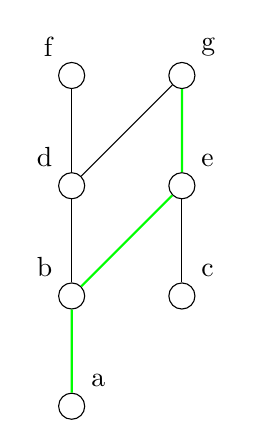
\begin{tikzpicture}[scale=.7]
  \node[circle, draw=black, text=black, label={135:f}] (f) at (0, 0) {};
  \node[circle, draw=black, text=black, label={45:g}] (g) at (2, 0) {};
  \node[circle, draw=black, text=black, label={135:d}] (d) at (0, -2) {};
  \node[circle, draw=black, text=black, label={45:e}] (e) at (2, -2) {};
  \node[circle, draw=black, text=black, label={135:b}] (b) at (0, -4) {};
  \node[circle, draw=black, text=black, label={45:c}] (c) at (2, -4) {};
  \node[circle, draw=black, text=black, label={45:a}] (a) at (0, -6) {};

  \draw [green, thick] (a) -- (b) -- (e) -- (g);
  \draw (b) -- (d) -- (f);
  \draw (c) -- (e);
  \draw (d) -- (g);
\end{tikzpicture}

% =============================================================================
%
% References
%
% =============================================================================

\chapter*{References}
\addcontentsline{toc}{chapter}{References}

\begin{itemize}
  \item $[1]$ \href{https://www.cambridge.org/core/books/introduction-to-lattices-and-order/946458CB6638AF86D85BA00F5787F4F4}{B. A. Davey, H. A. Priestley: \it{Introduction to Lattices and Order}}
\end{itemize}

\end{document}
